\documentclass{standalone}

\usepackage{tikz-cd}
\usepackage{satex}

\begin{document}
$\twocell{((1->1)["f"])}$

\begin{tikzcd}
  \twocell{((1->1)["f"])}
\end{tikzcd}

\begin{tikzcd}
  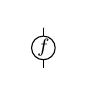
\begin{tikzpicture}[baseline=(current bounding box.center),yscale=-1,scale=0.5,every path/.style={join=round,cap=round}]
    \draw (0.000000,0.000000) -- (0.000000,0.500000);
    \draw (0.000000,0.500000) -- (0.000000,1.000000);
    \filldraw[fill=white] (0.000000,0.500000) ellipse (0.300000 and 0.300000);
    \draw (0.000000,0.500000) node[shape=rectangle,anchor=center] {$\scriptstyle f$};
  \end{tikzpicture}
\end{tikzcd}
\end{document}
